\clearpage
%//==============================--@--==============================//%
\subsection[2.3 Eletronic Mail (email)]{\hspace*{0.075 em}\raisebox{0.2 em}{$\pmb{\drsh}$} Eletronic Mail (email)}
\label{subsec:eletronic-mail}

%//==============================--@--==============================//%
\subsubsection[2.3.1 Simple Mail Transfer Protocol (SMTP)]{$\pmb{\rightarrow}$ Simple Mail Transfer Protocol (SMTP)}

\begin{theo}[\underline{Simple Mail Transfer Protocol (SMTP)}]{teo/def:SMTP}\label{teo/def:SMTP}
    ``SMTP is the principal application-layer protocol for Internet electronic mail. It uses the reliable data transfer service of TCP to transfer mail from the sender’s mail server to the recipient’s mail server. As with most application-layer protocols, SMTP has two sides: a client side, which executes on the sender’s mail server, and a server side, which executes on the recipient’s mail server."\cite{Kurose2017}
\end{theo}

\noindent \textbf{Nota:} ``SMTP restricts the body (not just the headers) of all mail messages to simple 7-bit ASCII'' \& ``does not normally use intermediate mail servers for sending mail, even when the two mail servers are located at opposite ends of the world.''´. Assim, se o servidor de destino estiver inativo, a receção da mensagem está dependente do reenvio por parte do servidor do utilizador, não permanecendo num servidor de resguardo temporário.

\definecolor{codegray}{rgb}{0.5,0.5,0.5}
\begin{lstlisting}[language=, title={Exemplo SMTP \protect\cite{slidesSobrinho}}, frame=tb, basicstyle=\footnotesize\ttfamily\color{codegray}]
S: 220 destino.pt
C: HELO origem.pt
S: 250 Hello origem.pt, pleased to meet you
C: MAIL FROM: fernando@origem.pt
S: 250 fernando@origem.pt ... Sender ok
C: RCPT TO: luis@destino.pt
S: 250 luis@destino.pt ... Recipient ok
C: DATA
S: 354 Enter mail, end with "." on a line by itself
C: From: fernando@origem.pt
C: To: luis@destino.pt
C:
C: Deus quer, o homem sonha, a obra nasce
C: .
S: 250 Message accepted for delivery
C: QUIT
S: 221 destino.pt closing connection
\end{lstlisting}

\begin{itemize}
    \item The client sends a message (``Deus quer, o homem sonha, a obra nasce'') from mail server \texttt{origem.pt} to mail server \texttt{destino.pt}.
    
    \item The client issued five commands: \texttt{HELO} (an abbreviation for HELLO), \texttt{MAIL FROM}, \texttt{RCPT TO}, \texttt{DATA}, and \texttt{QUIT}.
    
    \item The client also sends a line consisting of a single period, which indicates the end of the message to the server.
    
    \item The server issues replies to each command, with each reply having a reply code and some (optional) English-language explanation (e.g.: \texttt{354 Enter mail, end with "." on a line by itself}).
    \item SMTP uses persistent connections: If the sending mail server has several messages to send to the same receiving mail server, it can send all of the messages over the same TCP connection.
    
    \item For each message, the client begins the process with a new \texttt{MAIL FROM: origem.pt}, designates the end of the message with an isolated period, and issues \texttt{QUIT} only after all messages have been sent.
\end{itemize}
%//==============================--@--==============================//%
\subsubsection[2.3.2 Formato da mensagem]{$\pmb{\rightarrow}$ Formato da mensagem}%miminhos :3
O formato típico atribuído ao cabeçalho de um email é:
\definecolor{codegray}{rgb}{0.5,0.5,0.5}
\begin{lstlisting}[language=, title={Exemplo do formato do cabeçalho de uma mensagem}, frame=tb, basicstyle=\footnotesize\ttfamily\color{codegray}]
From: fernando@origem.pt
To: luis@destino.edu
Subject: Tenho em mim todos os sonhos do mundo
\end{lstlisting}
\noindent O cabeçalho é seguido de uma linha em branco e do corpo do email.

\vspace{1 em}
\noindent \textbf{Nota:} ``It is important to note that these header lines are different from the SMTP commands (even though they contain some common words such as “from” and “to”). The commands in that section were part of the SMTP handshaking protocol; the header lines examined in this section are part of
the mail message itself."\cite{Kurose2017}

%//==============================--@--==============================//%
\subsubsection[2.3.3 Mail access protocol]{$\pmb{\rightarrow}$ Mail access protocol}

\begin{figure}[H]
    \centering
    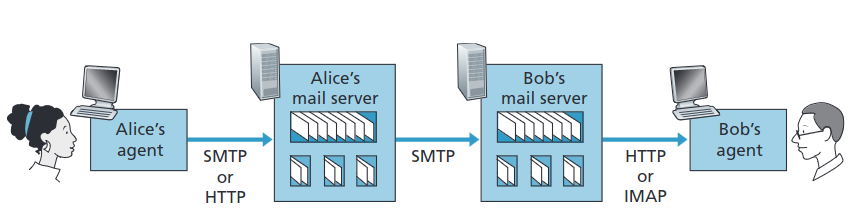
\includegraphics[width = 1\linewidth]{img/2/email-server.png}
    \caption{Protocolos de \textit{push} e \textit{pull}}
    \label{fig:email-server}
\end{figure}

\begin{itemize}
    \item Alice’s user agent uses SMTP or HTTP to deliver the e-mail
message into her mail server, then Alice’s mail server uses SMTP (as an SMTP client) to relay the e-mail message to Bob’s mail server. The two step procedure allows Alice’s mail server to repeatedly try to send the message to Bob’s mail server, until Bob’s mail server becomes operational.

    \item On the other hand, if Bob is using Web-based e-mail or a smartphone app (such as Gmail), then the user agent will use HTTP (since obtaining the messages is a pull operation, whereas SMTP is a push protocol) to retrieve Bob’s e-mail. This case requires Bob’s mail server to have an HTTP interface as well as an SMTP interface (to communicate with Alice’s mail server).
\end{itemize}

\noindent The alternative method, typically used with mail clients such as Microsoft Outlook, is to use the Internet Mail Access Protocol (IMAP). Both the HTTP and IMAP approaches allow Bob to manage folders, maintained in Bob’s mail server.
\renewcommand*{\thefootnote}{\fnsymbol{footnote}}
\footnotetext[4]{%
    \noindent \textbf{Internet Message Access Protocol (IMAP):} managing and accessing email messages on a remote.
    
    \vspace{-1em}
    \begin{enumerate}
        \item \textbf{Server-based Storage:} IMAP stores email messages on a remote server, allowing users to access their emails from multiple devices without needing to download messages locally.
        \item \textbf{Folder Organization:} Users can create, rename, and delete folders to organize their emails.
        \item \textbf{Selective Retrieval:} IMAP supports downloading only email headers or specific parts of a message, conserving bandwidth and improving efficiency.
        \item \textbf{Synchronization:} Changes made to emails, such as marking messages as read or moving them between folders, are synchronized with the server, ensuring a consistent view across all devices.
    \end{enumerate}
}
\renewcommand*{\thefootnote}{\arabic{footnote}}
%//==============================--@--==============================//%